\documentclass[letterpaper, 10 pt, conference]{ieeeconf}  % Comment this line out if you need a4paper

%\documentclass[a4paper, 10pt, conference]{ieeeconf}      % Use this line for a4 paper

\IEEEoverridecommandlockouts                              % This command is only needed if 
                                                          % you want to use the \thanks command

\overrideIEEEmargins                                      % Needed to meet printer requirements.

%In case you encounter the following error:
%Error 1010 The PDF file may be corrupt (unable to open PDF file) OR
%Error 1000 An error occurred while parsing a contents stream. Unable to analyze the PDF file.
%This is a known problem with pdfLaTeX conversion filter. The file cannot be opened with acrobat reader
%Please use one of the alternatives below to circumvent this error by uncommenting one or the other
%\pdfobjcompresslevel=0
%\pdfminorversion=4

% See the \addtolength command later in the file to balance the column lengths
% on the last page of the document

% The following packages can be found on http:\\www.ctan.org
\usepackage{graphics} % for pdf, bitmapped graphics files
\usepackage{epsfig} % for postscript graphics files
\usepackage{mathptmx} % assumes new font selection scheme installed
\usepackage{times} % assumes new font selection scheme installed
\usepackage{amsmath} % assumes amsmath package installed
\usepackage{amssymb}  % assumes amsmath package installed

\title{\LARGE \bf
Preparation of Papers for IEEE Sponsored Conferences \& Symposia
}

\author{Albert Author$^{1}$ and Bernard D. Researcher$^{2}$}

\begin{document}

\maketitle
\thispagestyle{empty}
\pagestyle{empty}


%%%%%%%%%%%%%%%%%%%%%%%%%%%%%%%%%%%%%%%%%%%%%%%%%%%%%%%%%%%%%%%%%%%%%%%%%%%%%%%%
\begin{abstract}
This electronic document is a live template. 
\end{abstract}
%%%%%%%%%%%%%%%%%%%%%%%%%%%%%%%%%%%%%%%%%%%%%%%%%%%%%%%%%%%%%%%%%%%%%%%%%%%%%%%%

\section{INTRODUCTION}
\subsection{Shared Space and Movement Efficiency}
In recent years, shared space, which is a kind of urban design has been increasingly introduced especially in some Europian urban areas. 

\subsection{The Effects of Minority to the Whole Movement Efficiency}
Text here.

\subsection{Brake Index}
In shared space, collision avoidane models which previous studies has developed might not be efficient because various road users (e.g., pedestrians, bicycles, and cars) coexist and there are no explicit rules for the priority.

\section{OBJECTIVE}
This study examined how the whole movements efficieny would change as the ratio of agents whose movement algorithms are different. We expected to find the threshold of the ratios of agents in the whole space that drastically change the movement effciiency. For example, considering the experiment carried by \cite{c2}, one qurater of whole agents could be one of the bottleneck; namely, when the number of cooperative agents reached the one qurater of the whole agents, movement efficiency drastically increased. Otherwise, there is also possibility that the raise of movement efficiency follows the linear change and the movement efficiency and the ratio of cooperative agents are in proportion. 

\section{METHOD}
To achive the objective of the study, we performed the computer simulation and measured the efficineny of the movements.  

\subsection{Simulation Environment}
The space of the simulation environment was set as a 500 by 500 pixel virtual space, where the simulation agents could move in two dimensions. Thus, the simulation environment was made to represent the shared space (Figure \ref{fig:sim_env}). The size of each agent was defiend as the radius of 5 pixel circle. In one trial, all agents moved 500 steps. All agnets' initial positions and initial velocities were randomized each time the simulation started.

\subsection{Avoidance Algorithms}
Based on the collision avoidance algorithms, agents were classified into two types.

For one of types, simple avoidance agent, their avoindace vectors were generated to the opposite direction of the other agents which approached within a 50 pixel. The size of avoidance vectors were fixed as either 1, 2, 3, 4, or 5 pixel in one trial. We call this type of agents as the simple avoidance agents.

For another type of agent, which we call as the dynamic avoidance agent, their avoidance vector were generated based on the braking index. When an agent approch to another agent within 50 pixel, the braking rate was calculated based on their relative positions and velocities, and their avoidance vectors were determined from 1 to 3 pixel. This way of avoidance enabled agents to avoid other agents considering how much potential danger they are facing; in safer situations, agents avoid slightly, on the contrary, in more dangerous situation, agents avoid widely not to collide each other. 

\subsection{Metrics of movement efficiency}
The movement efficiency was measured from two perspectives: completion time and number of collisions. Completion times was calculated as the mean steps for each agent took to reach their goals, where each agent has goals to reach. After they reached their goals, another goal was set so that all agent always has the destination to go. Number of collisions is the mean of how many times each agent collided with other agents. When more than two agents approached each other at the distance of closer than 5 pixel, those agents' collision count was added. These two metrics were expected to be inverse-ratioal to each other because we assume that when agents avoid others more widely, their completion time should be longer and vice versa. Completion time and the number of collisions were calculated for each agent and all agents' values were averaged.

\subsection{Change of the ratios of Dynamic Avoidance Agents}
To verify how the change of ratios of dynamic avoidance agents affects the whole movement efficiency, we performed simulations varying the ratios of dynamic avoidance agnets in the whole simulation environment. The variations of ratios were a range of 0 to 1. Therefore, when the ratio was 0, all agents in the environment move based on the simple avoidance algorithm, and when the ratio was 1, all agents in the environment moved based on the dynamic aovidance algorithm. We performed 20 trials of the simulation per ratio and all trials' completion time and number of collisions were averaged.

\begin{figure}[thpb]
   \centering
   \framebox{\parbox{3in}{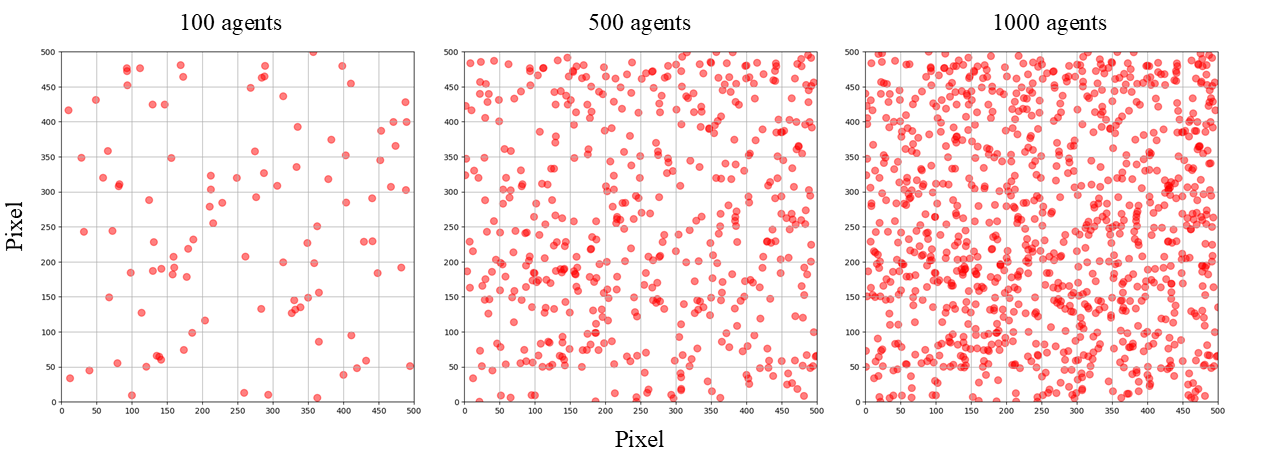
\includegraphics[scale=0.4]{figs/overview_simulation.png}}}
   \caption{Overview of the simulation environment}
   \label{fig:sim_env}
\end{figure}

\section{RESULTS} 
Figure \ref{fig:result_time} shows the transition of the mean of all agents' completion time. In case of that simple avoid vec is smaller than 2 px, completion time increase as the proprotions of the dynamic agent increases. For other cases, where the simple avoid vec is more than 3 px, the completion time decreases as the dynamic agent increases.

\begin{figure}[thpb]
   \centering
   \framebox{\parbox{3in}{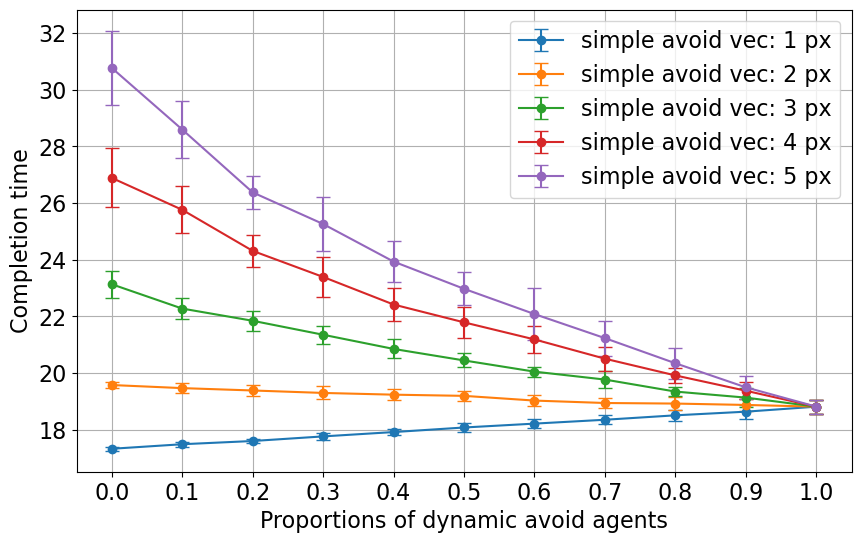
\includegraphics[scale=0.34]{figs/completion_time.png}}}
   \caption{Transitions of completion time as the ratio of dynamic avoidance agent increase.}
   \label{fig:result_time}
\end{figure}

Figure \ref{fig:result_collisions} shows the transition of the mean of all agents' number of collisions. On the contrary to the completion time, when the simple avoidance vectors are smaller than 2 px, the number of collision decreases as the ratio of the dynamic avoidance agents increases; conversely, when the vectors are larger than 3 px, the number of collisions increased. 

\begin{figure}[thpb]
   \centering
   \framebox{\parbox{3in}{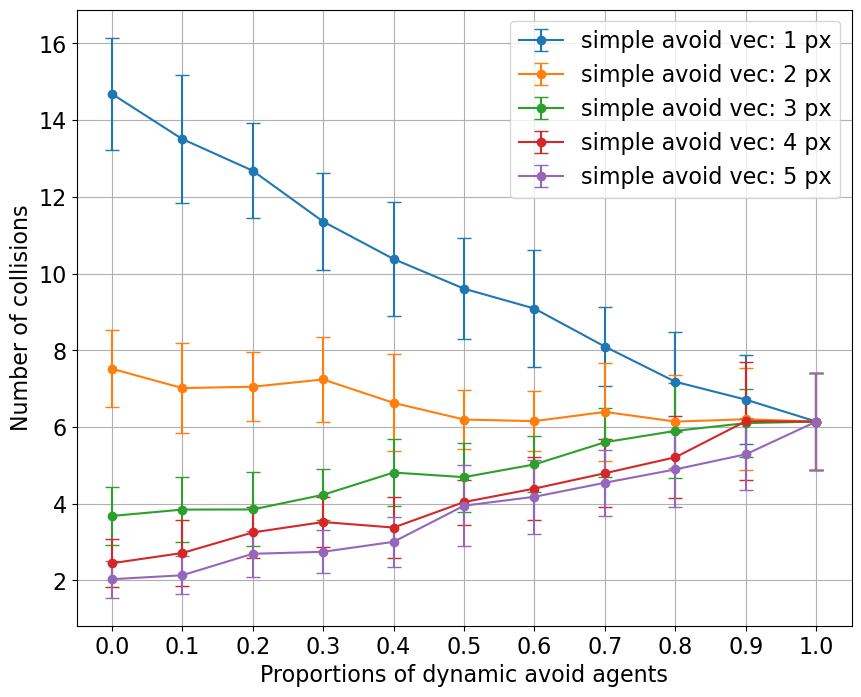
\includegraphics[scale=0.34]{figs/number_of_collisions.png}}}
   \caption{Transitions of number of collisiosn as the ratio of dynamic avoidance agent increase.}
   \label{fig:result_collisions}
\end{figure}

\subsection{Transition of Movement Efficiency}

\subsection{Units}

\begin{itemize}
\item Use either SI (MKS) or CGS as primary units. 
\end{itemize}

\section{DISCUSSION}
As the resutls showed, the trade-off between the completion time and the number of collisions was observed when increasing the ratio of the dynamic avoid agents, except when the simple avoid vector is 2 px. For the simualtion environment where the simple avoidance vector is small, (i.e., 1 px) the increasing of the dynamic agents increased the completion time and decreased the number of collisions. While dynamic avoidance agents decreased the completion time and increased the number of collisions. 
Because we consider the dynamic avoidance agnets as the cooperative movements in the environment, it is possible to say that these results imply that cooperative movements do not always beneficial to the movement efficiency, but there is the situation where the cooperative movements is beneficial to both the completion time and the number of collisions.


\section{TABLE}

\subsection{Equations}

The equations are an exception to the prescribed specifications of this template. 

$$z
\alpha + \beta = \chi \eqno{(1)}
$$

Note that the equation is centered using a center tab stop. 

Use this sample document as your LaTeX source file to create your document. 

\subsection{Figures and Tables}
Positioning Figures and Tables.

\begin{table}[h]
\caption{An Example of a Table}
\label{table_example}
\begin{center}
\begin{tabular}{|c||c|}
\hline
One & Two\\
\hline
Three & Four\\
\hline
\end{tabular}
\end{center}
\end{table}


Figure Labels: Use 8 point Times New Roman for Figure labels. 

\section{CONCLUSIONS}
A conclusion section is not required. Although a conclusion may review the main points of the paper, do not replicate the abstract as the conclusion. A conclusion might elaborate on the importance of the work or suggest applications and extensions. 

\addtolength{\textheight}{-12cm}  

\section*{APPENDIX}
Appendixes should appear before the acknowledgment.

\section*{ACKNOWLEDGMENT}
The preferred spelling of the word on the first page. We cited \cite{c2}.

\begin{thebibliography}{99}

\bibitem{c1} G. O. Young, Synthetic structure of industrial plastics (Book style with paper title and editor), in Plastics, 2nd ed. vol. 3, J. Peters, Ed.  New York: McGraw-Hill, 1964, pp. 1564.
\bibitem{c2} Matsubayashi, S., Miwa, K., Terai, H., and Ninomiya, Y. (2024). Index of braking behaviour in two dimensions within risk perception. Transportation research part F: traffic psychology and behaviour, 102, 164-176.

\end{thebibliography}

\end{document}
